\documentclass[12pt,a4paper,twoside]{article}
\usepackage[latin1]{inputenc}
\usepackage{amsmath}
\usepackage{amsfonts}
\usepackage{amssymb}
\usepackage{color}
\usepackage{listings}
\usepackage{graphicx}
\usepackage{upgreek}

\author{David Hogg, Rory Holmes}
\title{Ubercalibration Simulations \\(Euclid)}
\date{Jan 2011}

\makeatletter
\def\maketitle{%
  \null
  \thispagestyle{empty}%
  \vfill
  \begin{center}\leavevmode
    \normalfont
    {\LARGE \@title\par}%
    \vskip 1cm
    {\Large \@author\par}%
    \vskip 1cm
    {\Large \@date\par}%
  \end{center}%
  \vfill
  \null
  \cleardoublepage
  }
\makeatother

\begin{document}
\maketitle

\section{Introduction}
These simulations... 

\section{General}

\subsection{Parameter File}

Simulation parameters are stored in the parameter.py file.

\subsection{General Functions}
The functions.py file contains two routine for converting between magnitudes and fluxes. ..

\section{Sky Catalog}
We create a fake sky, based on realistic star densities, between a magnitude of 19 to 22.5. The upper and lower limits are defined based the saturation and 10$\upsigma$ limits for a single Euclid exposure. Star's are generated with random coordinates (within the sky region being investigated) and with a random magnitude according to the following powerlaw:
\begin{equation}
\frac{1}{N} \frac{dN}{dm} = A + B m
\end{equation}

The \textit{Transformation Method} is used generate random numbers with the appropriate probability density function. 

\begin{equation}
\log_{10} \frac{\Delta N}{\Delta m} = A + B m
\end{equation}

\begin{equation}
\frac{d N}{d m} =10^ {A + B m}
\end{equation}

prob dist function int = 1

\begin{equation}
\frac{d N}{d m} =10^ {A + B m}
\end{equation}

\begin{figure}[ht]
\begin{center}
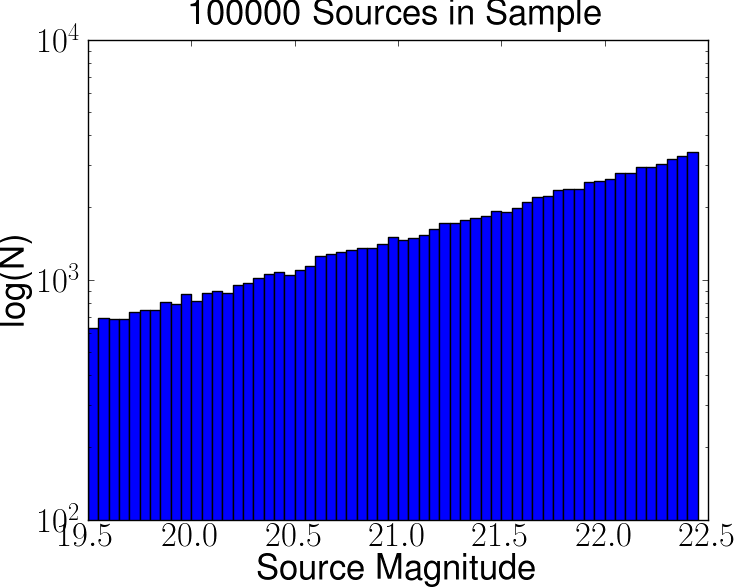
\includegraphics[width=\textwidth]{source_mag_histogram.png}
\end{center}
\caption{A histogram of the generated star magnitudes. The number of stars is given by... XX \label{fig:source_magnitude}}
\end{figure}

\begin{figure}[ht]
\begin{center}
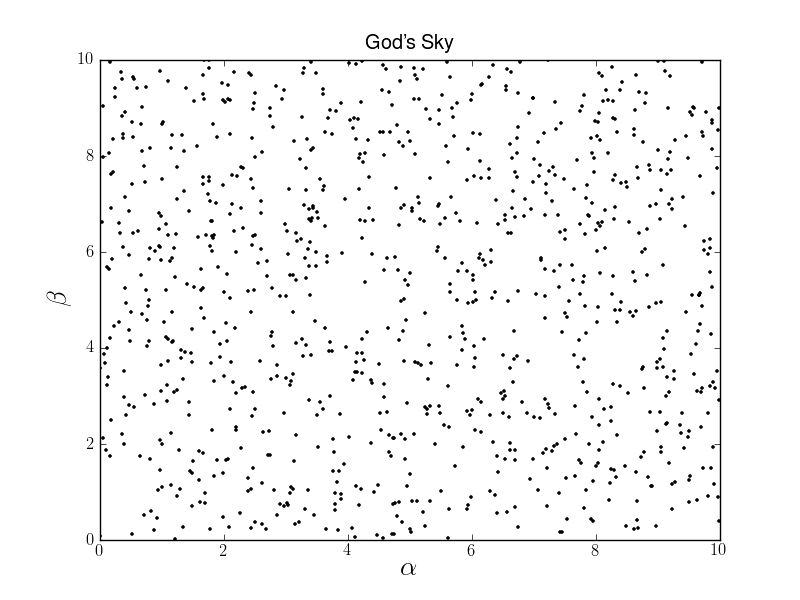
\includegraphics[width=\textwidth]{gods_sky.png}
\end{center}
\caption{A small subset of the simulated sky catalog produced. \label{fig:gods_sky}}
\end{figure}

The random number generate is given the same seed, so that the same simulated sky is produced each time the routine is called.


\section{Camera Model}

\subsection{Sky to Focal Plane Coordinate Transformations}

\subsection{Uncertainty Inverse-Variance}
\begin{figure}[ht]
\begin{center}
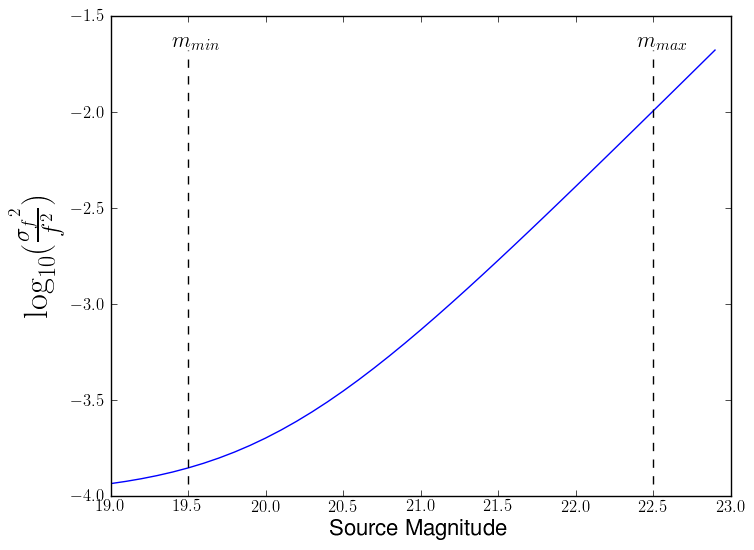
\includegraphics[width=\textwidth]{flux_uncertainty_variance.png}
\end{center}
\caption{XX UPDATE \label{fig:flux_uncertainty}}
\end{figure}
\subsection{Catalog to Measured Flux Conversion}

\section{Ubercalibration}
The ubercalibration procedure works in two sub-steps: (i) the star fluxes are refined based on the latest flat-field estimate (\textit{s\_step}) and (ii) the flat-field parameters are refined based on the latest star flux estimates (\textit{q\_step}). We iterate these steps until the parameters converge. In our notation $j$ refers to the iteration step. 

Our flat-field is defined by a set of parameters $\vec{q}$. After the $j$th iteration, the flat-field parameters will be indexed as $\vec{q_j}$. The individual star measurements are defined as $c_i$ (``counts''), where each $i$ corresponds to a exposure number $n$, a specific star with ID number $k$ and a focal plane position $\vec{x}$.

XX Our model is

\begin{equation}
c_i = f(\vec{x_i} | \vec{q_j}) . s_{kj} + e_{ij}
\end{equation}

where $s_k$ is the true flux from star $k$ and our error is drawn from the Normal Distribution $e_{ij} = N(e|0,{\sigma_i}^2)$.

\subsection{Star Flux Refinement: \textbf{\textit{s\_step}}}
The flux estimates, $s_k$, for each star can be considered individually. At step $j$ we can refine a star's flux estimate (to $s_{kj+1}$) by minimizing the error function with the latest flat-field parameters:

\begin{equation}
\chi^2_{k} = \sum_{i \in \mathcal{O}(k)} \frac{(c_i-f_{ij}s_{kj})^2}{{\sigma_i}^2}
\end{equation}

\begin{equation}
\frac{d\chi^2_{k}}{d s_{kj}} = \sum_{i \in \mathcal{O}(k)} \frac{-2 f_{ij} (c_i-f_{ij}s_{kj+1})}{{\sigma_i}^2} = 0
\end{equation}

\begin{equation}
\Rightarrow \sum_{i \in \mathcal{O}(k)} \frac{f_{ij} c_i}{{\sigma_i}^2}= \sum_{i \in \mathcal{O}(k)} \frac{f_{ij}^2 s_{kj+1}}{{\sigma_i}^2}
\end{equation}

\begin{equation}
\Rightarrow s_{kj+1} = {\sum_{i \in \mathcal{O}(k)} \frac{f_{ij} c_i}{{\sigma_i}^2}}/{\sum_{i \in \mathcal{O}(k)} \frac{f_{ij}^2}{{\sigma_i}^2}} \label{eqn:s_step}
\end{equation}

The standard uncertainty inverse variance on $s_{kj+1}$ is given by the denominator in Eqn \ref{eqn:s_step}.

\subsection{Flat-Field Refinement: \textbf{\textit{p\_step}}}
The flat-field parameters can now be refined with the latest star flux estimates. To do this we minimize the error function for all measurements with respect to the flat-field parameters.

\begin{equation}
\chi^2 = \sum_{i} \frac{(c_i-f_{ij}s_{kj+1})^2}{{\sigma_i}^2}
\end{equation}

\begin{equation}
f_{ij} = \sum_{l = 1}^L q_{lj} g_l(\vec{x_i})
\end{equation}

\begin{equation}
\chi^2 = \sum_{i} \frac{(c_i- s_{kj+1} \sum_{l = 1}^L q_{lj} g_l(\vec{x_i}))^2}{{\sigma_i}^2}
\end{equation}

\begin{equation}
\frac{d\chi^2}{dq_{lj}} = \sum_{i} \frac{-2 g_l(\vec{x_i}) s_{kj+1} (c_i- s_{kj+1} \sum_{l' = 1}^{L'} q_{l'j} g_{l'}(\vec{x_i}))}{{\sigma_i}^2} = 0
\end{equation}

\begin{equation}
\sum_{i} \frac{g_l(\vec{x_i}) s_{kj+1} c_i}{{\sigma_i}^2} = \sum_{i} \frac{g_l(\vec{x_i}) s_{kj+1}^2 \sum_{l' = 1}^{L'} q_{l'j+1} g_{l'}(\vec{x_i})}{{\sigma_i}^2}
\end{equation}

\end{document}
